\documentclass[a4paper,twoside,kulak]{kulakreport}
% LATEX CLASSES
% Standaard: article, report, book, beamer, sciposter
% Huisstijl: kulakarticle, kulakreport, kulakbook, kulakbeamer, kulaksciposter

% PREAMBULE
% dit is het gedeelte tussen \documentclass en de \begin{document}
% hier worden extra pakketten geladen en instellingen gemaakt

% Essentiële pakketten aan het begin van de preambule om correct compileren mogelijk te maken
\usepackage[utf8]{inputenc} % Correct vreemde symbolen inlezen
\usepackage[dutch]{babel}   % Nederlandstalige regels voor woordafbreking
\usepackage[T1]{fontenc}    % Correct vreemde symbolen weergeven
\usepackage{float}
\usepackage{gensymb}
\usepackage{lscape}
\usepackage{rotating}
\usepackage{pdfpages}
\usepackage[square,numbers]{natbib}
\usepackage{siunitx}
\bibliographystyle{abbrvnat}

% Instellingen voor titelpagina, kop- en voettekst
% In een standaard article-document zijn er minder mogelijkheden
\faculty{Wetenschap \& Technologie Kulak}
\group{}
\title{Human Pose Estimation:\\Toepassing}
\subtitle{}
\author{Isaac venus\\Stan Vanhecke\\Mathieu Vanooteghem}
% \\Stan Vanhecke\\Mathieu Vanooteghem
\emailaddress{isaac.venus@student.kuleuven.be}
% \\stan.vanhecke@student.kuleuven.be\\mathieu.vanooteghem@student.kuleuven.be
\institute{KU Leuven Kulak, Wetenschap \& Technologie}
\date{Titularis: Koen Van Den Abeele\\Begleider: Jens Goemare\\Academiejaar 2020 -- 2021}
\address{
   KU Leuven Kulak           \\
   Wetenschap \& Technologie \\
   Etienne Sabbelaan 53, 8500 Kortrijk             \\
   Tel.\ +32 56 24 60 20     \\
   \href{mailto:\theemailaddress}{\texttt{\theemailaddress}}
   }

\begin{document} % hier begint de eigenlijke inhoud van het document

\titlepage

\tableofcontents

\chapter*{Inleiding}
Aan materiaal in de medische wereld hangt steeds een stevig prijskaartje, dus vroegen wij ons af hoe we dit wat lichter kunnen maken voor de portemonnee. Wat natuurlijk niet mag is het gebruik van hoogtechnologische medische apparatuur. In de plaats daarvan wordt gekozen voor technologie die iedereen ter beschikking heeft: een laptop of een smartphone. We moeten dus software schrijven die met de elektronica die we al hebben kan werken. In dit verslag richten wij ons op \emph{human pose estimation} (HPE), of lichaamspositiebepaling. We gebruiken hiervoor de open-source HPE software Openpose die via neurale netwerken de positie van een persoon schat op een foto en de coördinaten van verschillende knooppunten in het menselijk lichaam teruggeeft waarmee we dan berekeningen kunnen uitvoeren. Ons doel is om Openpose te gebruiken voor medische toepassingen. In dit verslag zullen we er twee uitwerken: het opvolgen van de revalidatie na een schouderoperatie en het bepalen van de optimale fietspositie om blessures te voorkomen. In beide gevallen kunnen we met behulp van HPE een goeie en goedkope oplossing aanbieden die gemakkelijk toegankelijk is voor iedereen.

\chapter{Theoretische achtergrond}
\section{HPE, revolutionair?}
\emph{Human pose estimation} is de laatste tijd veel geëvolueerd naar een heel gebruiksvriendelijke vorm. Vroeger waren hiervoor hoogtechnologische opstellingen met mensen in speciale pakken en veel rekenkracht nodig. Nu zijn een foto en een laptop voldoende om de posities van zelfs meerdere personen in hetzelfde beeld tegelijkertijd te bepalen. Dit allemaal door de gigantische vooruitgang op vlak van artificiele intelligentie en neurale netwerken.

	\begin{figure}[H]
		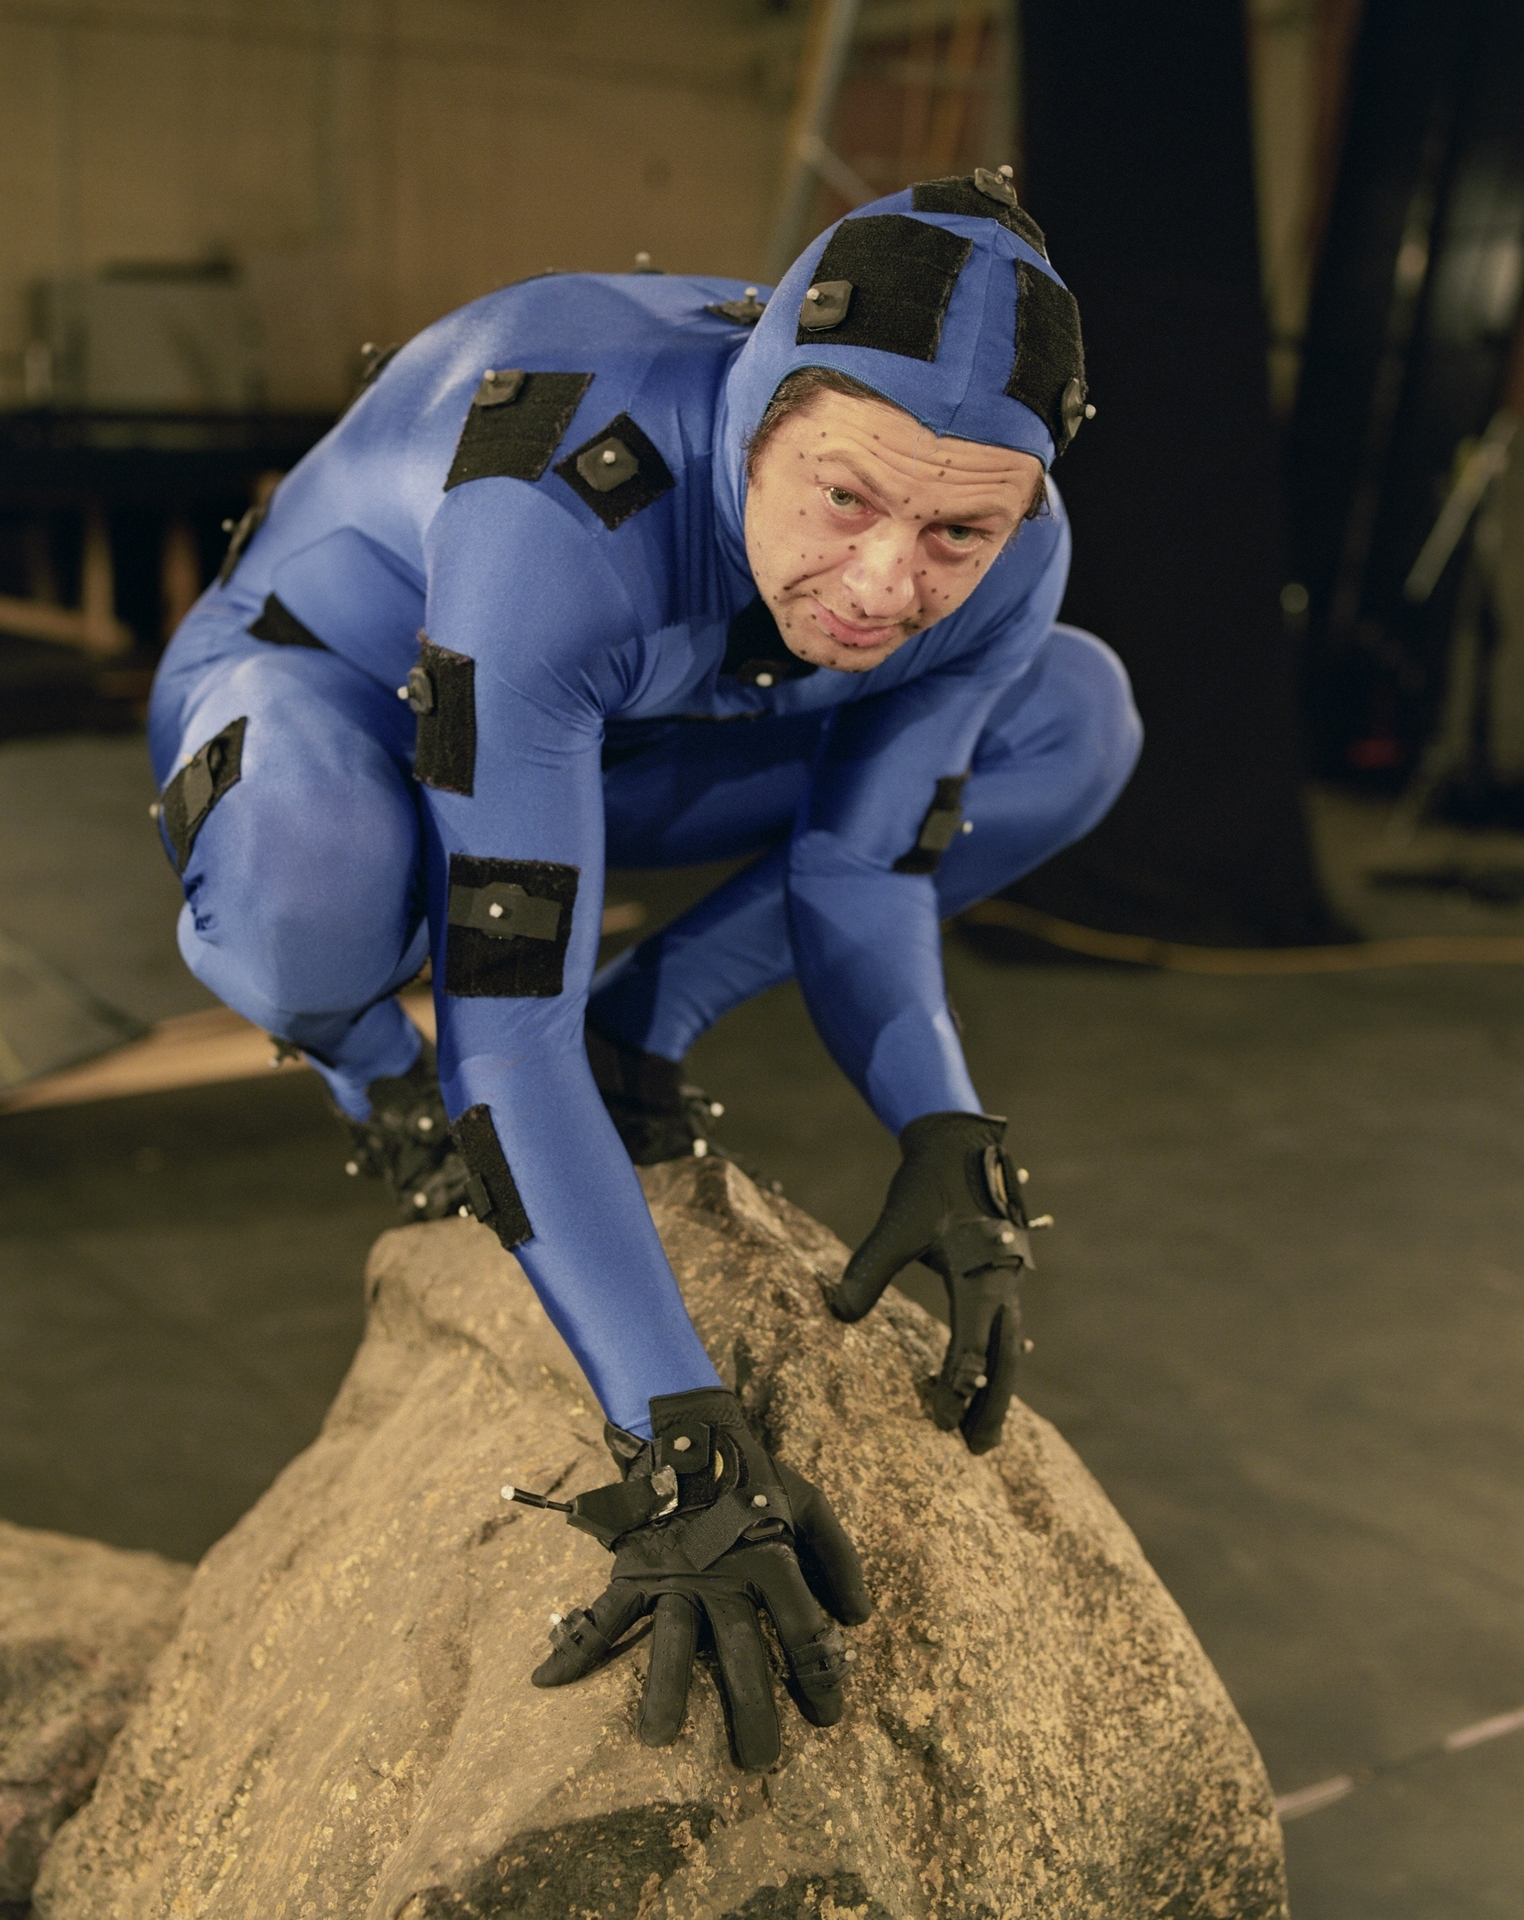
\includegraphics[width=.4\textwidth]{3D_motion_capture}
		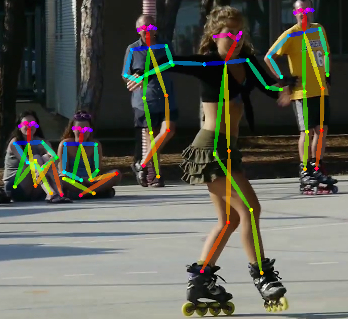
\includegraphics[width=.55\textwidth]{HPE_voorbeeld}
		\caption{Bij grote productiehuizen wordt de positie bepaald door middel van een 3D motion capture pak (links), maar tegenwoordig is HPE een veel goedkopere en gemakkelijkere oplossing (rechts).
		(afbeeldingen van https://www.pinterest.com/pin/718324209297102981/ en https://beyondminds.ai/an-overview-of-human-pose-estimation-with-deep-learning/}
	\end{figure}

\section{Openpose}
Openpose is een open-source programma dat \emph{human pose estimations} kan doen. Openpose is grotendeels geprogrammeerd in C++ maar heeft een uitstekende Python API. Dit programma onderscheidt zich van andere HPE programma's in de manier waarop het beelden met meerdere personen kan verwerken. De meeste voorgaande programma's waren maar in staat om met één persoon te werken of lokaliseerden eerst alle personen op de foto om nadien individueel hun positie te bepalen. Bij Openpose is het anders, het programma kan synchroon de positie van alle personen bepalen in de foto \cite{openpose}.
\subsection{Werking}
Openpose berekent eerst voor alle lichaamsdelen een heatmap. Dat zijn de locaties met het meeste kans dat het lichaamsdeel zich daar bevindt. Op basis daarvan kan hij dan de coördinaten bepalen \cite{heatmaps}.

\section{Neurale netwerken}
Een (artificieel) neuraal netwerk of ANN is een netwerk geïnspireerd op een biologisch neuraal netwerk zoals dat voorkomt in hersenen, met als doel deze iets te doen leren. Het ANN is opgebouwd uit artificiële neuronen die een neuron in een brein moeten voorstellen. Al de neuronen zijn verbonden met andere neuronen en kunnen signalen uitsturen en ontvangen. In een ANN zijn de signalen getallen en kan elk neuron een bepaalde bewerking uitvoeren op een binnenkomend signaal om deze verder te sturen. Elke connectie heeft ook een gewicht dat bepaalt hoe sterk het signaal is dat hij uitstuurt. Dit gewicht past zich aan als het neuraal netwerk leert. 

\subsection{Opbouw van een neuraal netwerk}
\paragraph{Neuronen}
Zoals er hierboven staat, is een artificieel neuron geïnspireerd op een neuron uit een brein. Elk neuron heeft een of meerdere inputs en één output die kan verzonden worden naar meerdere andere neuronen. De input van een neuron kan ofwel komen van de data die in het neuraal netwerk wordt gestoken of van andere neuronen. De output van de output neuronen is wat uit het programma komt. Om de output van een neuron te berekenen neem je de gewogen som van de inputs, met als gewicht de waarden van de connecties. Daarbij wordt ook nog eens een bias of vertekening opgeteld.

\paragraph{Connecties}
Om te kunnen leren moet het natuurlijk mogelijk zijn om de data door te geven van het ene neuron naar het andere. Dit verloopt via een “connectie” die een bepaald gewicht heeft dat de sterkte en daarmee ook het belang van een bepaalde connectie weergeeft.

\paragraph{Lagen}
Een neuraal netwerk bestaat uit meerdere lagen van neuronen, meer bepaald de \emph{input layer}, \emph{hidden layers} en \emph{output layer} \ref{netwerk}. Zoals de namen wel duidelijk maken geef je de data aan de \emph{input layer} en komen de berekende waarden uit de \emph{ouput layer}. Daartussen zijn er eventueel \emph{hidden layers}. Tussen twee lagen zijn er meerdere manieren van connecties tussen de neuronen mogelijk.

\begin{figure}
	\begin{center}
		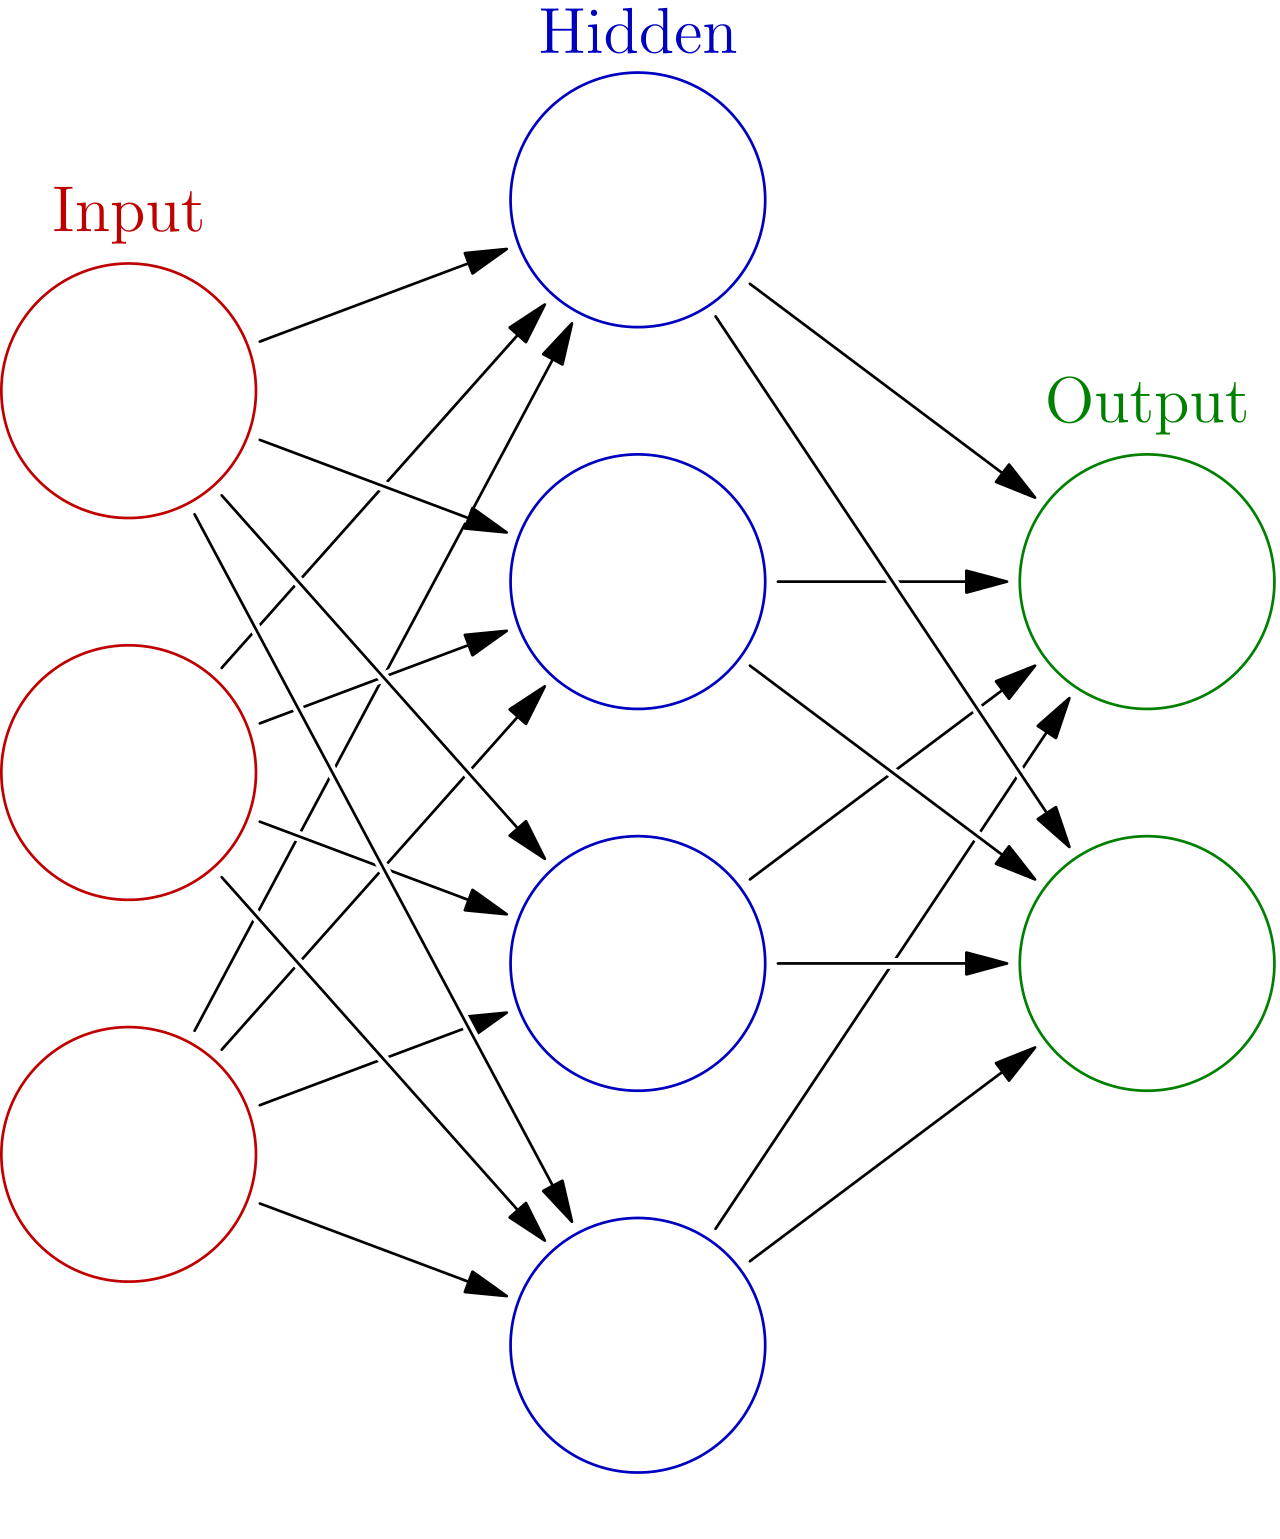
\includegraphics[width=8cm]{netwerk.png}
	\end{center}
	\caption{Voorbeeld van een neuraal netwerk. (afbeelding van wikipedia.org)}
	\label{netwerk}
\end{figure}

\subsection{Trainen van een neuraal netwerk}
Bij het programmeren van een neuraal netwerk weet je natuurlijk niet wat de gewichten zijn van alle connecties. Je moet het model dus doen leren. Dit doe je door de gewichten (over meerdere leercycli) aan te passen zodat de output zo goed mogelijk past bij het gewenste resultaat. Er zal altijd een bepaalde fout op de output zitten dus het model gaat nooit perfect zijn. Het trainen van een model is gedaan als de fout op de output niet meer verkleint en dus een minimum heeft bereikt. Het aanpassen van de gewichten gebeurt met een zekere \emph{learning rate}. Dit bepaalt de grootte van de correcties die gebeuren bij de gewichten. Bij een grote \emph{learning rate} kan je model sneller klaar zijn met leren, maar is er meer kans op een grotere fout op de output. Een kleine \emph{learning rate} zal het trainen vertragen maar je uiteindelijke resultaat zal beter zijn. Openpose is getraind met twee datasets \cite{openpose}: de COCO dataset, die bestaat uit meer dan 100.000 beelden en meer dan 1.000.000 \emph{keypoints}, en de MPII dataset.



\chapter{Toepassingen}
Zoals eerder al gezegd zullen we ons focussen op toepassingen in de medische wereld waarop HPE kan toegepast worden. Wij kunnen dan een goedkope oplossing ontwikkelen voor die toepassingen. Hierbij testen we mogelijke problemen en analyseren we of dit  een goede optie is. We proberen dit dan allemaal op een methodische manier uit te werken, waarbij we een specifiek geval steeds breder gaan bekijken.


Een eerste toepassing is het opvolgen van de revalidatie na een schouderoperatie. Met een foto gemaakt met een gsm kunnen we een analyse uitvoeren van de beweging van de schouder na de operatie en dan doorheen de revalidatie evalueren.

Een tweede en uitgebreidere toepassing is het analyseren van de positie op de fiets. Veel amateurwielrenners hebben een slechte houding op de fiets en een professionele bikefitting kost al snel een paar honderd euro. Via lichaamspositiebepaling kunnen wij met een simpele foto de positie bepalen op de fiets en dan correcties voorstellen. Dit is een goedkope oplossing die voor een zeer breed publiek inzetbaar is. Voor professionele wielrenners zal dit wel waarschijnlijk niet voldoende zijn, maar voor een amateur kan dit een goedkoop alternatief zijn.



\section{Toepassing 1: opvolgen van revalidatie na schouderoperatie}
\subsection{Bepalen van de hoek tussen arm en lichaam}

We willen meten hoe ver een persoon zijn arm kan roteren voor de opvolging van de revalidatie na een schouderoperatie. Hiervoor kunnen we de hoek tussen het opperarmbeen en een ander lichaamsdeel bepalen. Op figuur \ref{fig:skelet} komt dat dus neer op de hoek bepalen tussen de lijnstukken [32] en [21] of tussen de lijnstukken [15] en [65]. Als we Openpose gebruiken om de positie te schatten van een persoon op een foto krijgen we als output de coördinaten van de verschillende knooppunten. Met deze coördinaten hebben we voldoende informatie om de hoek te berekenen en zo objectieve informatie te krijgen over het verloop van de revalidatie.


Bij een foto vanuit vooraanzicht kunnen we berekenen hoe ver de patiënt zijn arm zijwaarts omhoog kan brengen. Bij een foto genomen vanuit zijaanzicht kunnen we berekenen hoe ver hij de arm vooruit kan omhoog steken. Het is wel belangrijk dat de foto altijd vanuit dezelfde positie wordt getrokken omdat er anders variatie kan zijn op de hoek.



\begin{figure}[H]
	\centering
	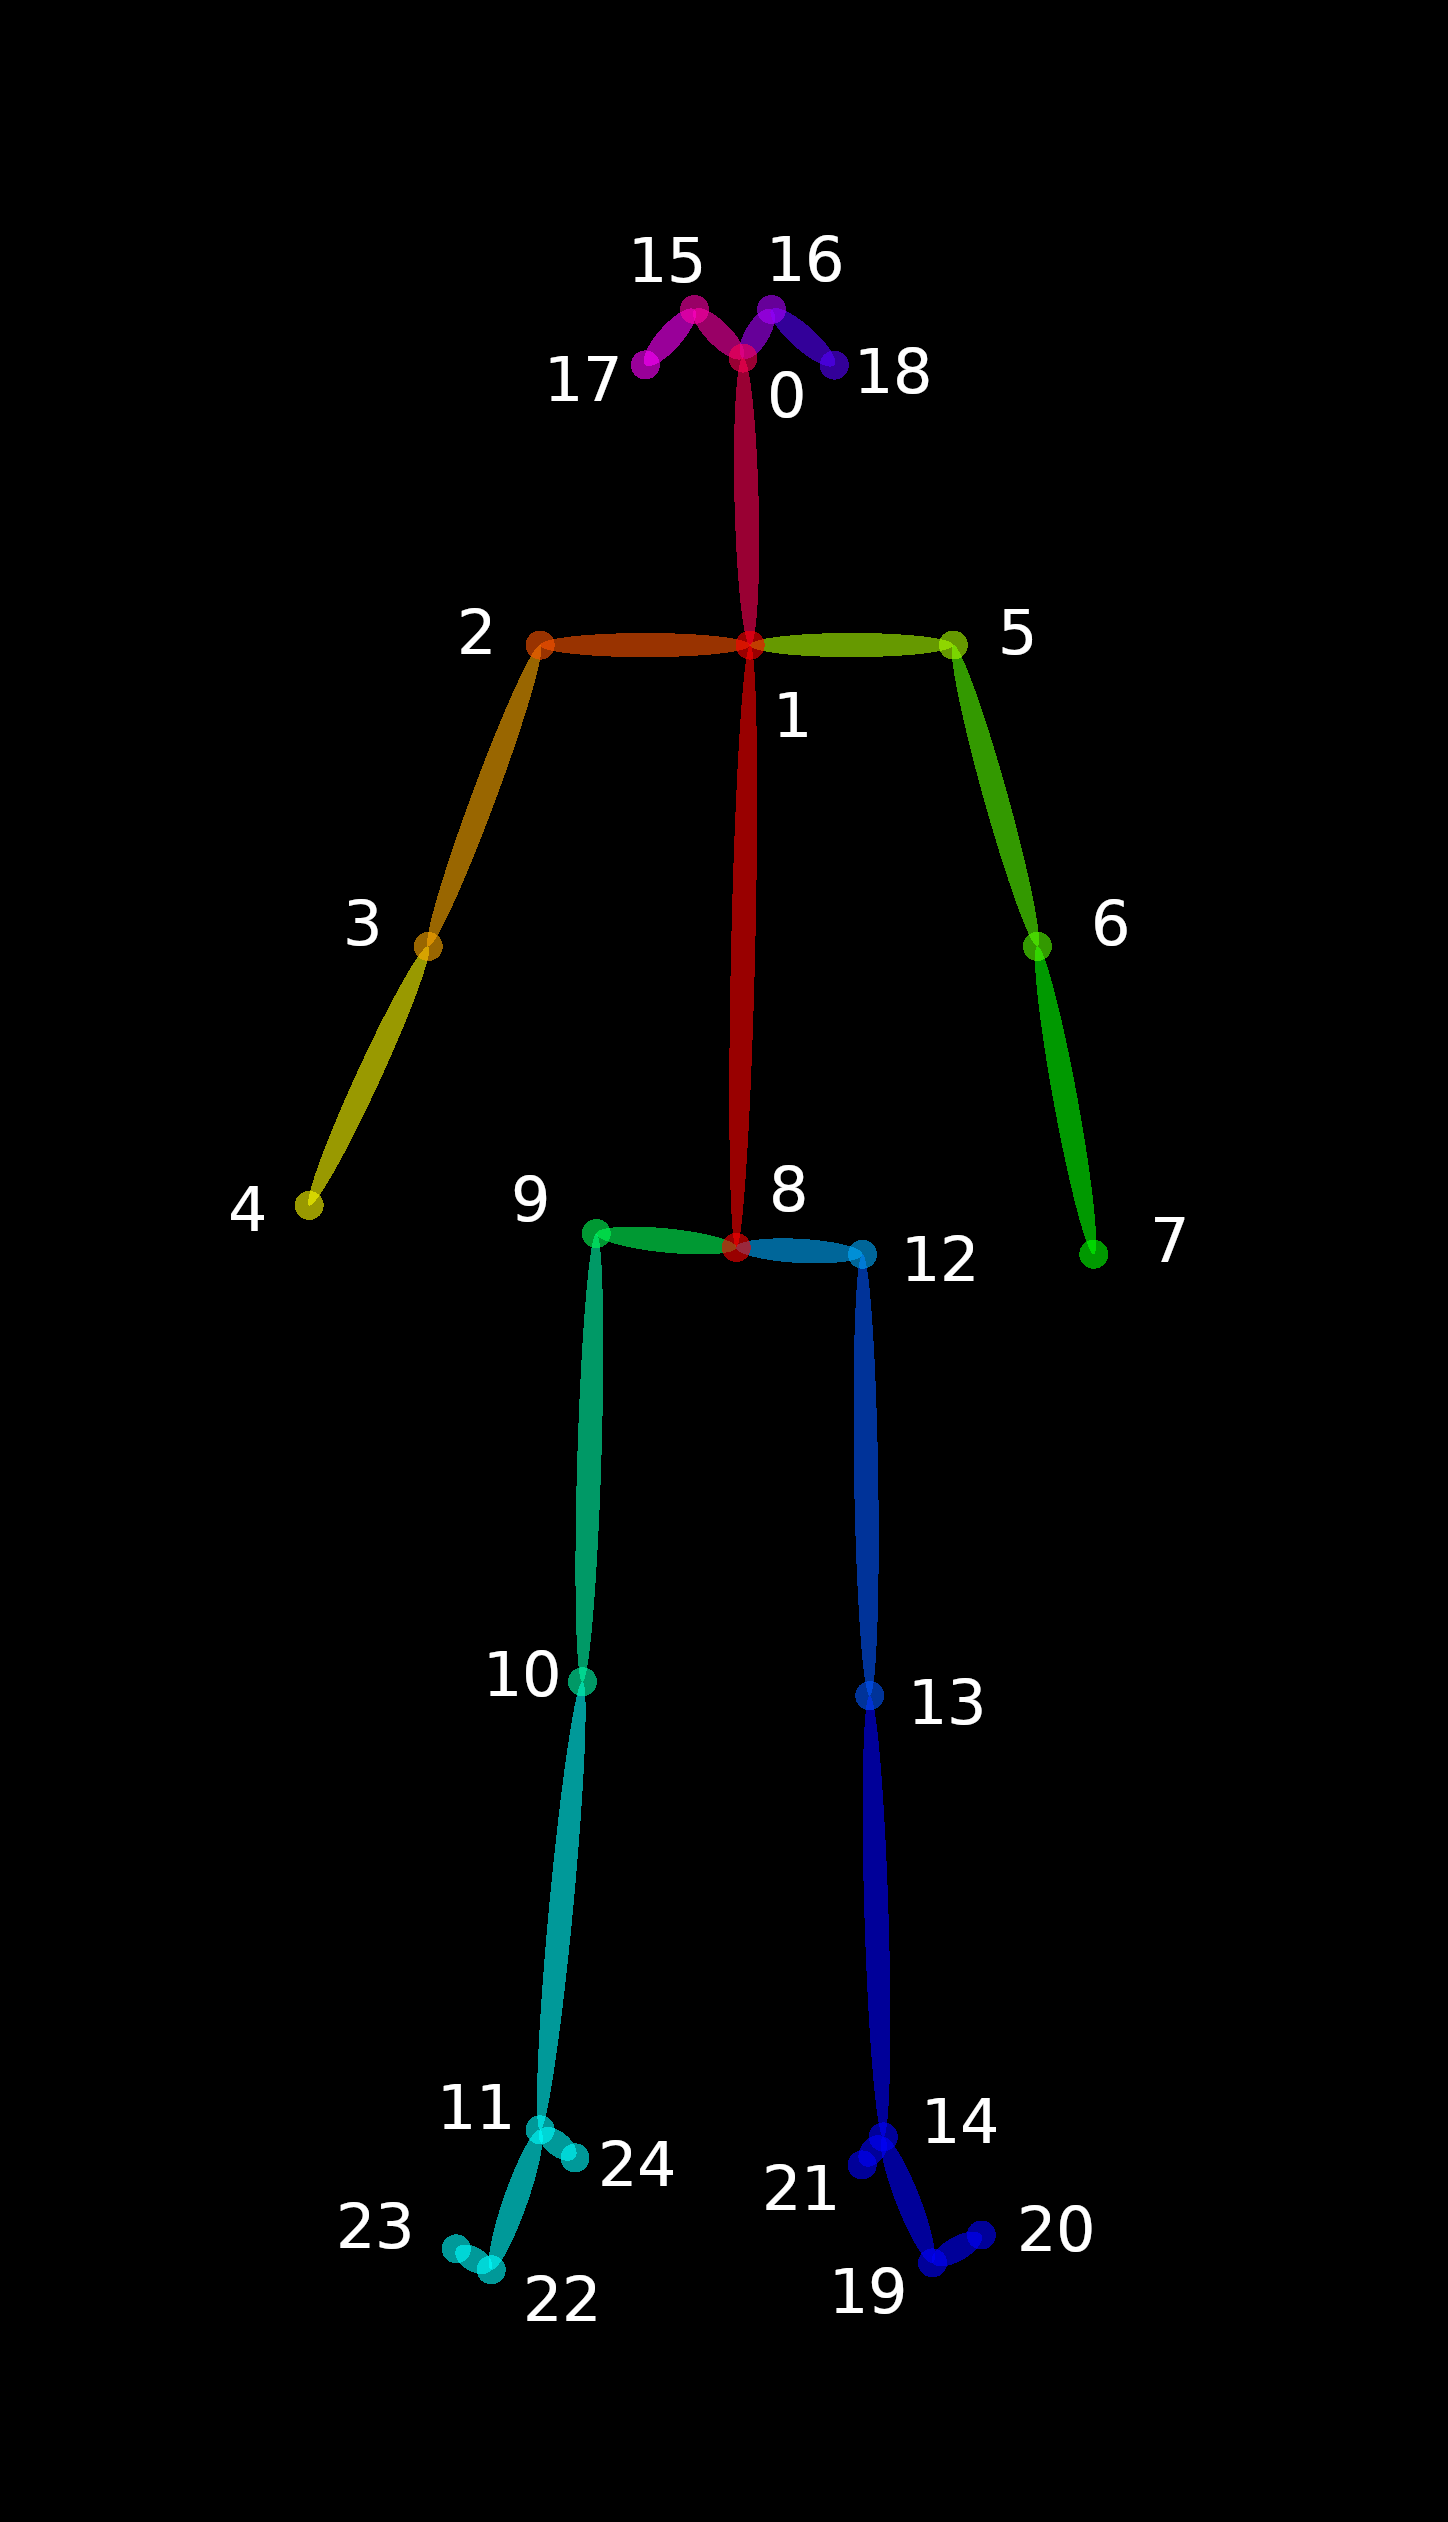
\includegraphics[width=.5\textwidth]{HPE_skelet}
	\caption{Voorstelling van de positie bepaald via Openpose (afbeelding van \href{https://github.com/CMU-Perceptual-Computing-Lab/openpose/blob/master/doc/output.md}{openpose})}
	\label{fig:skelet}
\end{figure}


\subsection{Voorlopige resultaten}

Via Openpose krijgen we de coördinaten van alle punten die openpose kan herkennen. Hiermee kunnen we dan verder onderzoek doen. Op dit moment zijn we in staat om hoeken tussen bepaalde lichaamsdelen te berekenen met als doel objectieve gegevens te bekomen tijdens bijvoorbeeld een revalidatie na een ongeval.

\paragraph{Wiskundige achtergrond}
Om de hoek tussen twee lichaamsdelen te berekenen gebruiken we de cosinusregel. Hier volgt een klein beetje duiding over hoe we die precies gebruiken (zie figuur \ref{cos}).\\

\begin{figure}[H]
	\begin{center}
		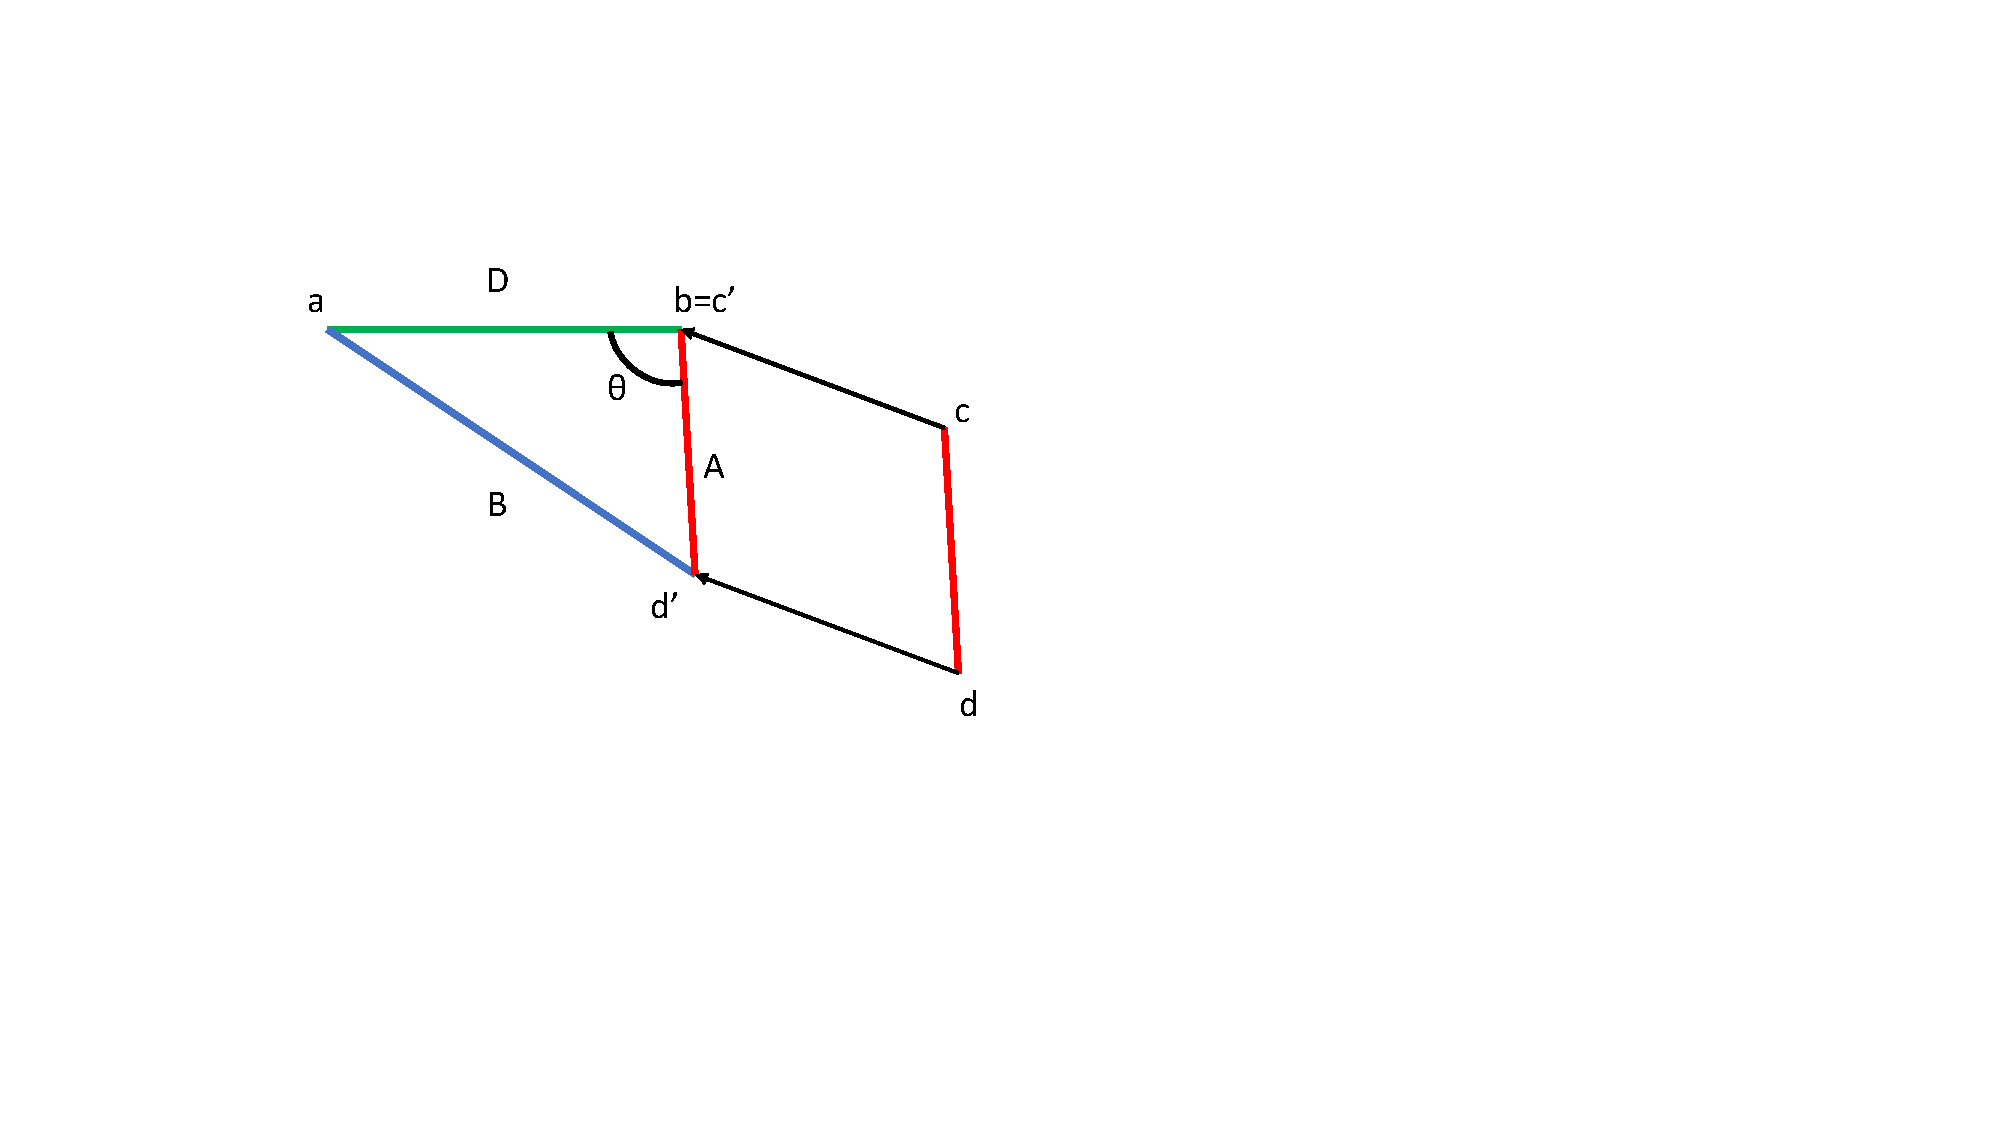
\includegraphics[width=10cm]{cos.pdf}
	\end{center}
	\caption{Hoek tussen 2 lichaamsdelen}
	\label{cos}
\end{figure}

We stellen \(a, b\) de coördinaten die het eerste lichaamsdeel afbakenen en \(c, d\) de coördinaten van het tweede lichaamsdeel. De hoek tussen de lichaamsdelen is dan de \(\theta\) van op de figuur. We kunnen gewoon de cosinusregel gebruiken om de hoek te bepalen als we \(c\) op \(b\) leggen. We krijgen dan
\[B^2 = A^2 + D^2 -2\cdot A\cdot D\cos\theta\]
en dus
\[\cos\theta = \frac{A^2 + B^2 - B^2}{2\cdot A\cdot D}\]
met
\[A = \sqrt{(d_x - c_x)^2 + (d_y - c_y)^2}\]
\[B = \sqrt{(b_x - a_x + d_x - c_x)^2 + (b_y - a_y + d_y - c_y)^2}\]
\[D = \sqrt{(b_x - a_x)^2 + (b_y - a_y)^2}\]
Als we dus de 4 coördinaten weten kunnen we de hoek bepalen.
\paragraph{Voorbeeld}
Een voorbeeld bij het bepalen van een hoek tussen de bovenarm en de romp is afbeelding \ref{samen}. Als we de hoek berekenen tussen de ruggengraat (rood) en het opperarmbeen(licht oranje) krijgen we als waarden:
\begin{itemize}
	\item Foto 1: 21.63 graden
	\item Foto 2: 78.06 graden
	\item Foto 3 130.00 graden
\end{itemize}
\begin{figure}
	\begin{center}
		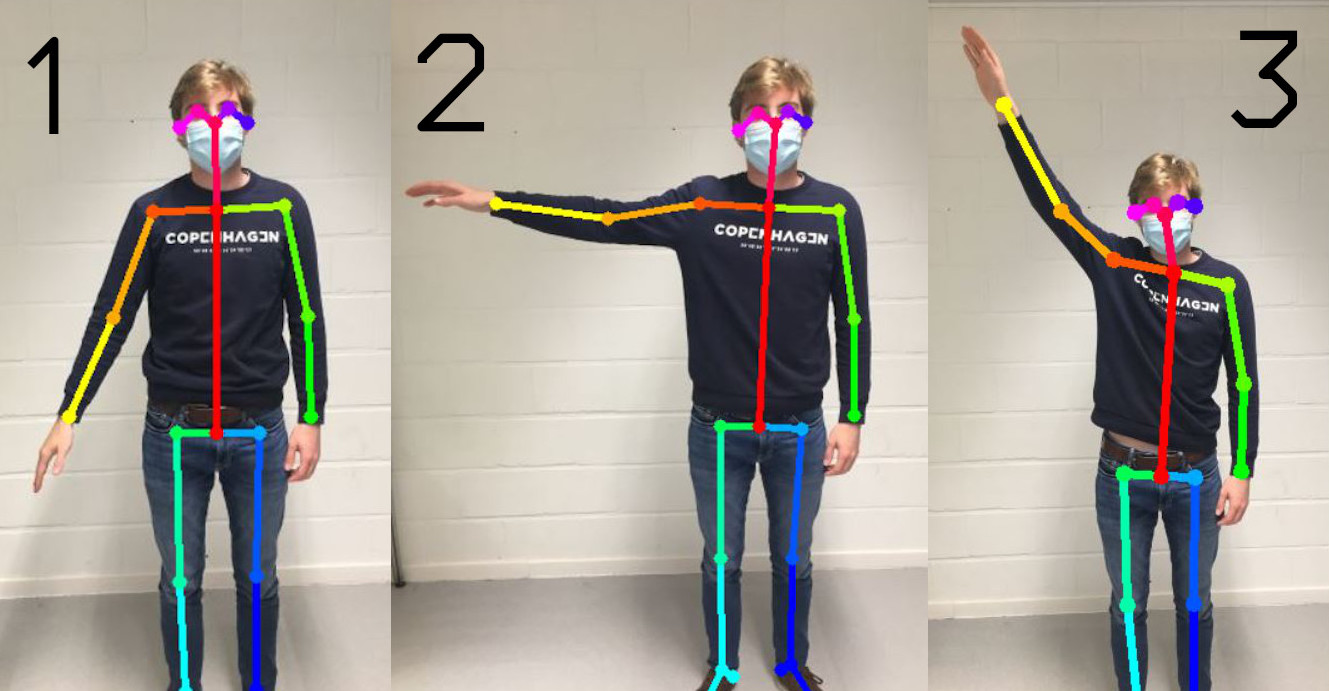
\includegraphics[width=12cm]{samen.jpg}
	\end{center}
	\caption{Voorbeeld bij het bepalen van een hoek.}
	\label{samen}
\end{figure}
\subsection{Voorlopige conclusies}
Door deze  toepassing weten we dat het relatief eenvoudig is om met Openpose zinvolle berekeningen te doen. Door de coördinaten die gegeven worden als output kunnen we gemakkelijk programma's schrijven die hiermee werken. Doordat Openpose werkt in 2D hebben we gemerkt dat de foto recht moet genomen worden. Als de hoek die we willen berekenen schuin afgebeeld staat op de inputfoto komt de berekening niet overeen met de werkelijke waarde van de hoek.


\section{Toepassing 2: fietspositie bepalen}
Voor de tweede toepassing willen we een goedkoper alternatief bieden voor een bikefitting. Hierbij worden er foto's getrokken van de persoon op de fiets en kunnen we dan op basis van de positie bepaald met Openpose eventuele correcties uitvoeren op de fiets.

Een bikefit is eigenlijk het analyseren en eventueel aanpassen van de positie op de fiets. Het belangrijkste doel daarvan is het voorkomen van blessures. Bij wielrenners die aan competitie doen heeft een bikefit ook als doel om een zo aerodynamisch mogelijke positie op de fiets aan te nemen. Ook kan een betere positie ervoor zorgen dat men een groter wattage kan leveren op de pedalen. Alleen maar voordelen dus.

\subsection{Principe}

Op Figuur \ref{fig:bikefit} staan enkele hoeken die voor de standaard persoon als optimaal gezien worden voor de positie op een koersfiets. Deze hoeken kunnen in een bepaald interval liggen afhankelijk van hoe flexibel de persoon is. Met behulp van Openpose berekenen we deze hoeken met als input een foto of video van de wielrenner vanuit een zo loodrecht mogelijk zijaanzicht. We hebben ondervonden dat de optimale positie voor de camera om een foto te nemen ongeveer 70 \si{cm} boven de grond is en 2\si{m} van de persoon verwijderd. Als de berekende hoeken te veel afwijken van wat voorop gesteld wordt, dan kunnen we een verbetering voorstellen. Dit kan een verhoging van het zadel zijn, een verandering van de lengte van de stuurpen, een verandering van de stuurhoogte... 


\begin{figure}[H]
	\centering
	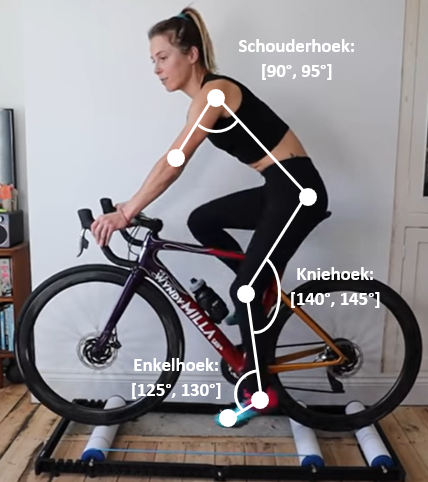
\includegraphics[width=\textwidth]{bikefit_hoeken_foto}
	\caption{Belangrijkste hoeken voor een optimale positie op de fiets (hoeken zijn gebaseerd op presentatie over bikefitting door Wolf Performance, bijgewoond door onze begeleider Jens Goemaere)}
	\label{fig:bikefit}
\end{figure}

\subsection{Algoritme voor wijzigen van de zadelhoogte}

We zullen beginnen met een algoritme te schrijven voor het veranderen van één parameter, namelijk de zadelhoogte. Voornamelijk de knie- en enkelhoek zullen veranderen als gevolg van een wijziging in zadelhoogte. Dit zal ook een klein effect hebben op de schouderhoek maar dit laten we hier voor het gemak achterwege. De mate waarin je de zadelhoogte kan wijzigen hangt af van de lengte van de zadelpen. Op de meeste zadelpennen staat de minimale diepte waarmee de pen in het frame moet zitten. Indien dit niet zo is, is de vuistregel dat de zadelpen minstens 90 \si{mm} diep in het frame moet zitten. Zet je zadel dus zeker niet hoger dan dat. Als je dit niet doet, bestaat de kans dat de zadelpen breekt.
In een eerste stap berekenen we enkel de kniehoek. We kijken initieel hoe groot die is. Indien de hoek tussen 140 \degree en 145 \degree ligt (zie Figuur \ref{fig:bikefit}), wordt er geen voorstel gedaan voor een wijziging van de zadelhoogte. Indien de hoek buiten dit interval ligt, berekent het algoritme met hoeveel pixels de y-coördinaat van het knooppunt van de heup moet wijzigen om de hoek in dit interval te krijgen. Vooraf wordt door het programma de lengte van bijvoorbeeld het bovenbeen gevraagd in \si{cm}. Via openpose kunnen we dan het aantal pixels berekenen tussen het knooppunt van de knie en de heup. Op die manier kunnen we de eenheid pixels overzetten naar \si{cm}. De output van het eerste is dan het aantal \si{cm} dat het algoritme voorstelt om het zadel te wijzigen. Een positief getal betekent verhogen, een negatief verlagen.

We breiden nu het algoritme uit zodat het ook de invloed van de wijziging van de zadelhoogte op de enkelhoek in rekening brengt. Deze is immers ook afhankelijk van de zadelhoogte. De optimale enkelhoek ligt tussen 125 \degree en 135 \degree. De moeilijkheid is nu om de zadelhoogte zodanig te kiezen zodat zowel de knie- als enkelhoek in het optimale interval liggen. De output is nog steeds een positief of negatief getal dat een voorstel doet voor het wijzigen van de zadelhoogte.

\subsection{Algoritme voor wijzigen van de stuurhoogte}

Als tweede parameter kijken we naar de stuurhoogte. Het aanpassen van de stuurhoogte heeft enkel invloed op de schouderhoek. Deze ligt in het optimale geval tussen 90 \degree en 95 \degree (zie Figuur \ref{fig:bikefit}). Het probleem is dat de voorvork meestal erg beperkt is in lengte. Bij de meeste amateur wielrenners wordt die afgezaagd net boven de stuurpen. Dit betekent dat er geen afstandsbus meer vanboven zit en het stuur dus niet meer verhoogd kan worden. Meestal zitten er wel nog afstandsbussen onder de stuurpen, dus het stuur kan dan wel nog verlaagd worden door één of meerdere afstandsbussen er vanonder uit te halen en boven de stuurpen te monteren. Omdat dit heel erg verschilt naargelang de fiets vragen we voor het algoritme als inputparameters hoeveel \si{cm} het stuur nog naar boven en naar beneden kan.

\subsection{Algoritme voor wijzigen van de stuurpenlengte}

Als laatste kijken we naar de invloed van de lengte van de stuurpen. Dit heeft ook enkel invloed op de schouderhoek. Het probleem is dat als we de lengte van de stuurpen willen aanpassen, we een nieuwe stuurpen moeten kopen. Daarom houden we dit als laatste aanpassing indien het wijzigen van de zadel- en stuurhoogte niet de gewenste hoeken opleveren. Er zijn ook bepaalde grenzen aan de lengte van een stuurpen. De minimale lengte is 40 \si{mm}, korter is bijna onmogelijk. Het maximum ligt rond de 140 \si{mm}, groter kan nog maar dat is heel uitzonderlijk. De output van het algoritme is de nieuwe vereiste stuurpenlengte.

\chapter{Vakintegratie}
Het is natuurlijk belangrijk om dit project een plaats te geven binnen onze opleiding ingenieurswetenschappen. We bekijken welke vakken uit de eerste 3 semesters van onze bachelor het meest gebruikt worden tijdens dit project. De belangrijkste link is met het vak begingselen van programmeren. In dit vak leerden we werken met Python en verworven we inzicht in het programmeren. Wat heel handig is, want tijdens ons project maken we veelvuldig gebruik van Python. Elk zelfgemaakt programma is geschreven in Python want Openpose heeft een uitstekende Python API. Verder maakt wiskunde ook een groot deel uit van ons project, want het berekenen van hoeken of afstanden kan niet zonder de wiskunde. We gebruiken hierbij kennis uit verschillende wiskundige vakken zoals, Analyse \& calclus en Lineaire algebra. Als laatste kunnen we Statistiek ook nog linken aan dit project aangezien Openpose enkel een schatting geeft van de lichaamspositie. Het werkt met \textit{heatmaps} en kiest per knooppunt dan het coördinaat met de hoogste kans. We gebruiken zelf geen statistische technieken, maar het helpt ons wel bij het begrijpen van Openpose.

\chapter{Planning}

\begin{landscape}
	\begin{figure}
		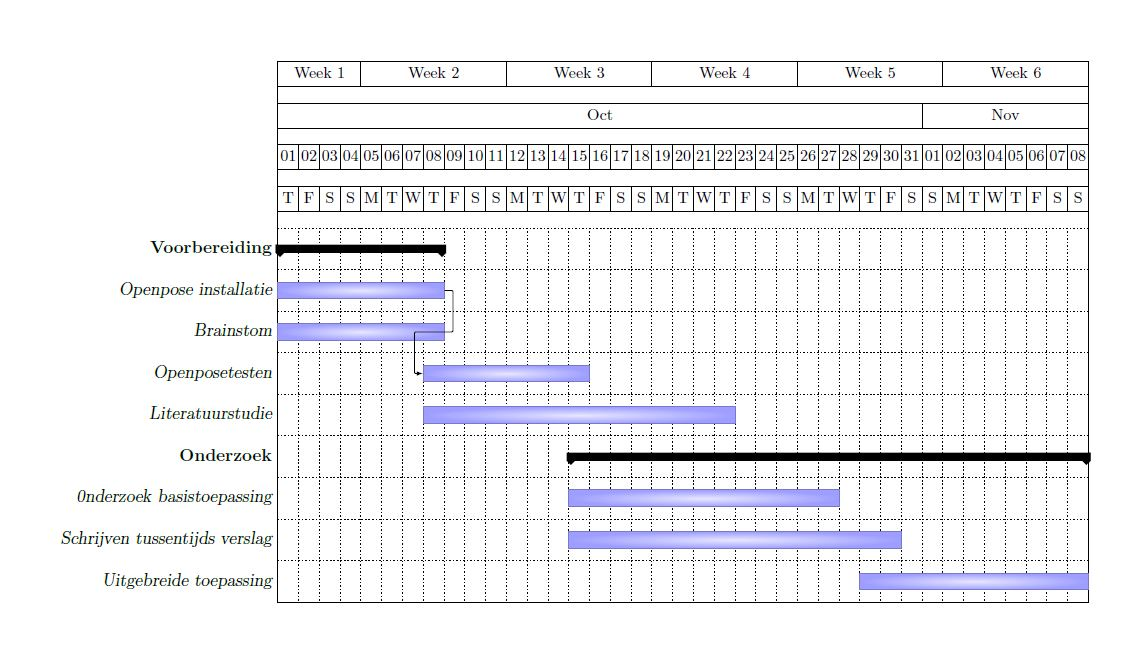
\includegraphics[width= 2\textwidth]{ganttchart_1}
	\end{figure}
	\begin{figure}
		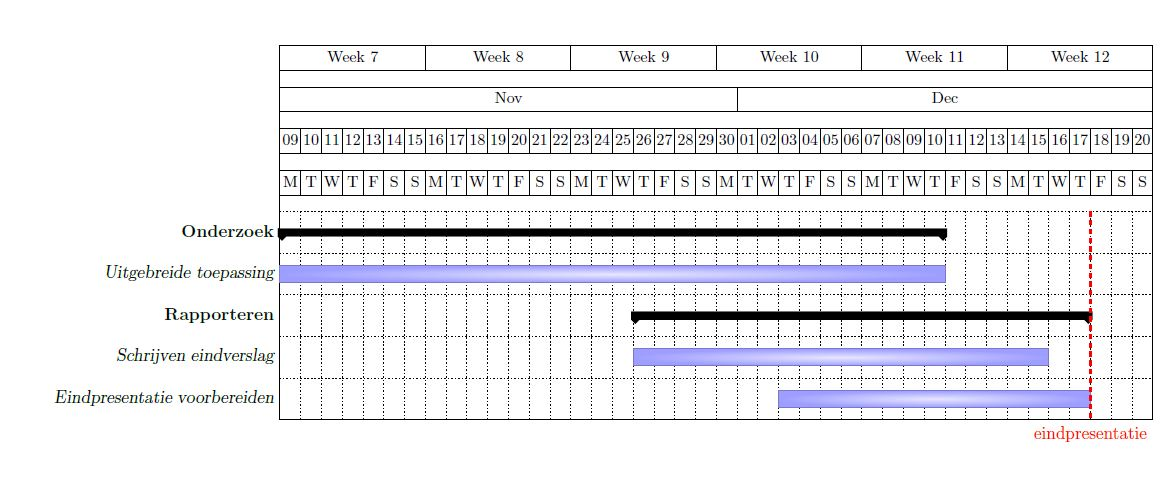
\includegraphics[width= 2\textwidth]{ganttchart_2}
	\end{figure}
\end{landscape}



\bibliographystyle{unsrt}
\bibliography{bibliografie}
%\printindex

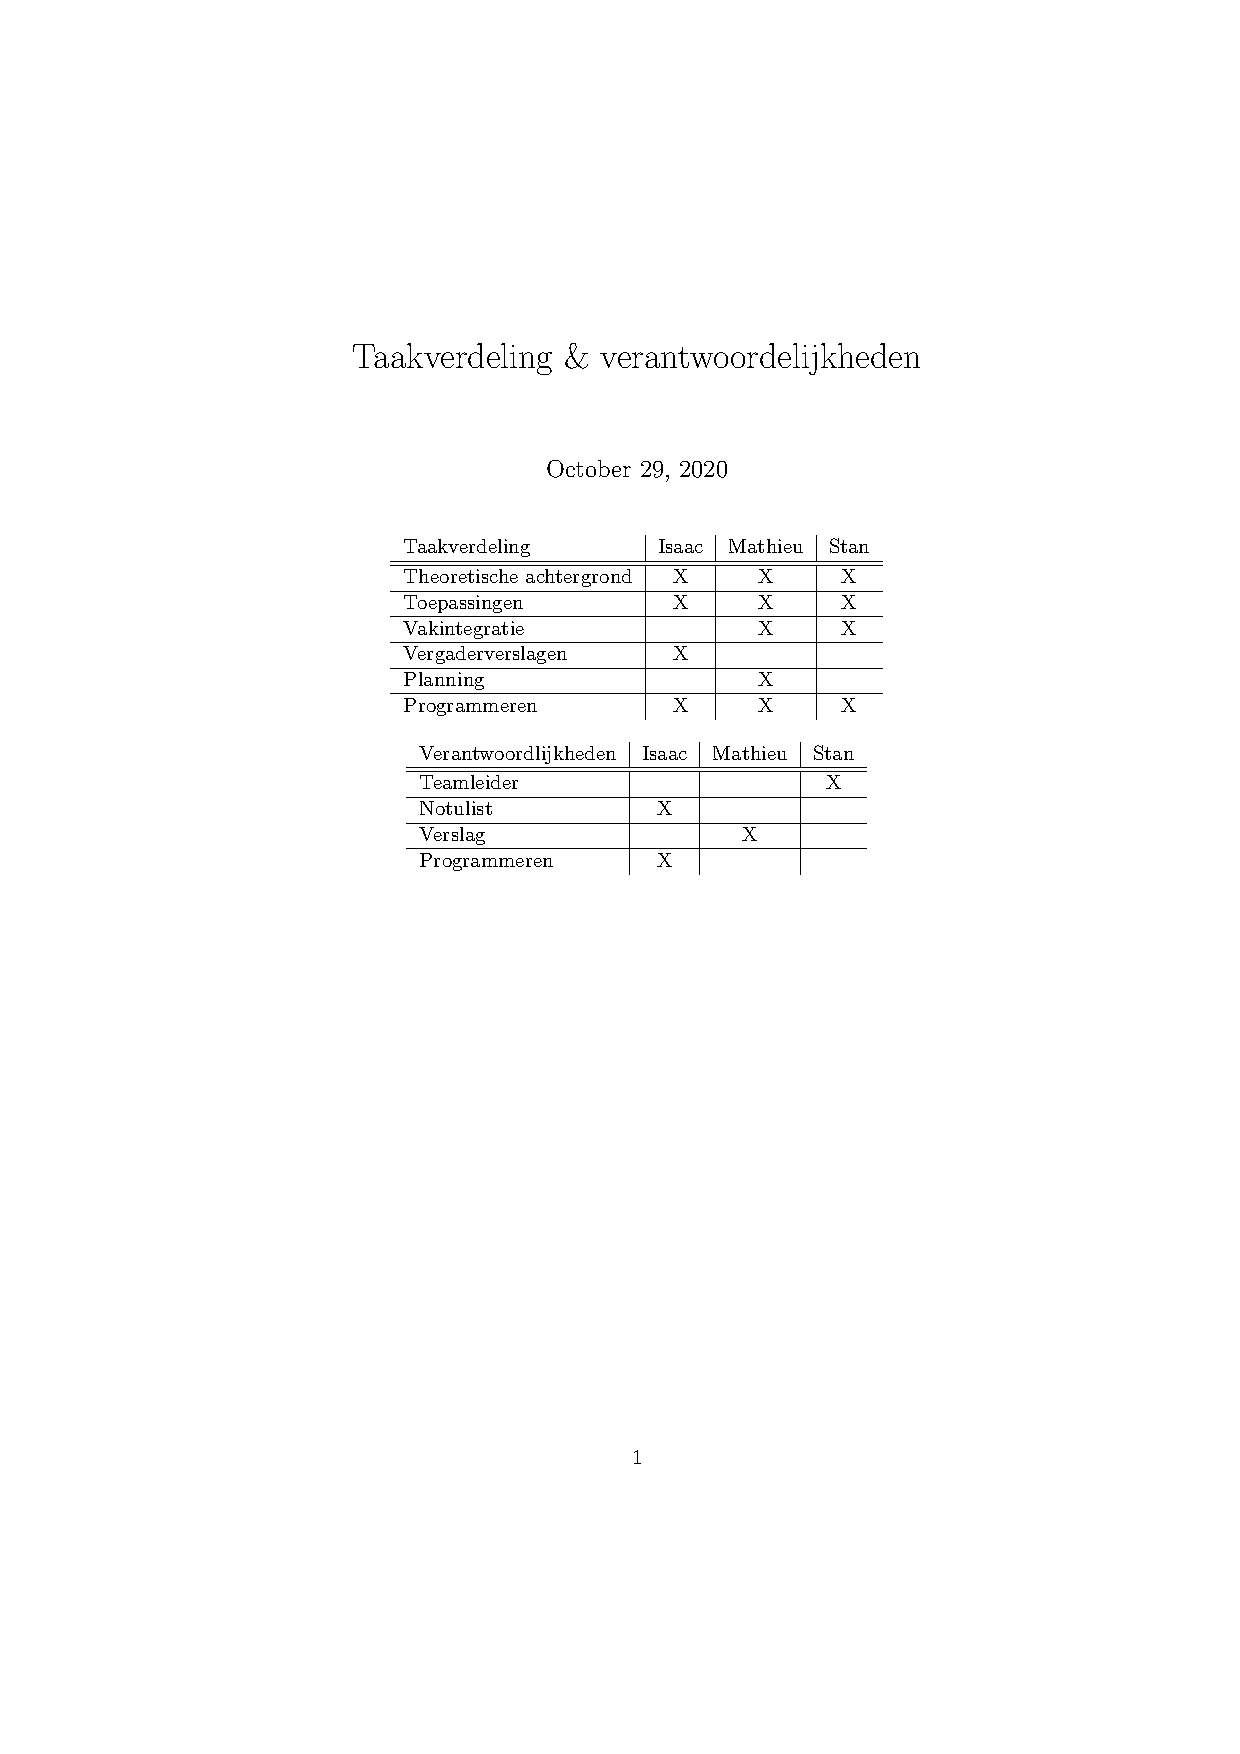
\includepdf{taakverdeling.pdf}

\end{document}